\lstinputlisting[style=cstyle]{Questions/Part2/prime2.c}

\subsubsection*{\underline{Experimental}}

\begin{tabular}{|c|c|c|c|c|c|c|c|c|c|c|}
\hline
N & 1000003 & 2000003 & 4000037 & 8000009 & 16000057 & 32000011 & 64000031 & 128000003 & 256000001 & 512000009 \\
\hline
\makecell{T(n)\\\(10^{-3}\)} & 1.676 & 3.247 & 6.842 & 13.009 & 25.376 & 52.545 & 102.985 & 205.319 & 397.85 & 802.53\\
\hline
\end{tabular}

\vspace{0.25cm}

\begin{tabular}{|c|c|c|}
    \hline
    N & 1024000009 & 2048000011\\
    \hline
    \makecell{T(n)\\\(10^{-3}\)}  & 1597.518 & 3200.743\\
    \hline
\end{tabular}

\vspace{0.5cm}

\begin{figure}[h!]
    \centering
    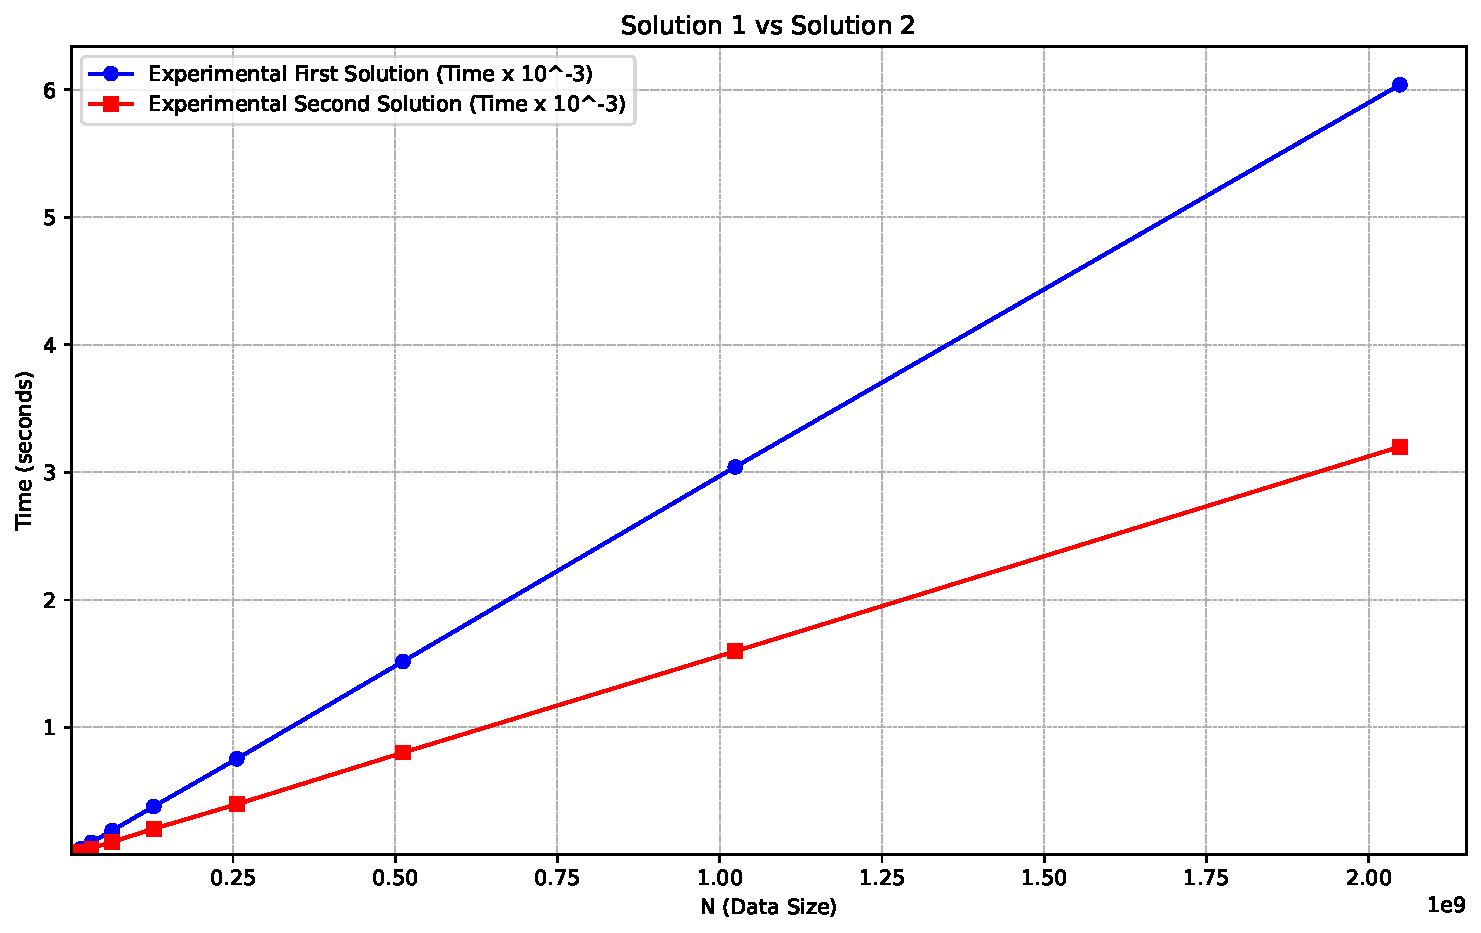
\includegraphics[width=0.85\textwidth]{Questions/Part2/plot.pdf}
    \label{fig:time_plot}
\end{figure}

\newpage

To Draw the plots i used the below python script :

\vspace{1cm}

\lstinputlisting[style=pythonstyle2,inputencoding=utf8]{Questions/Part2/draw.py}

\vspace{1cm}

\begin{prettyBox}{Observation}{greenPlot}
We notice that the second solution takes about half time of the first solution therefore the second solution
is more efficient
\end{prettyBox}
